\section{Фильтрация изображений с периодичностью}

Айоу, АКа, вот вам ... картинка с гугл диска, которая мне очень приглянулась.

\begin{figure}[ht!]
    \centering
    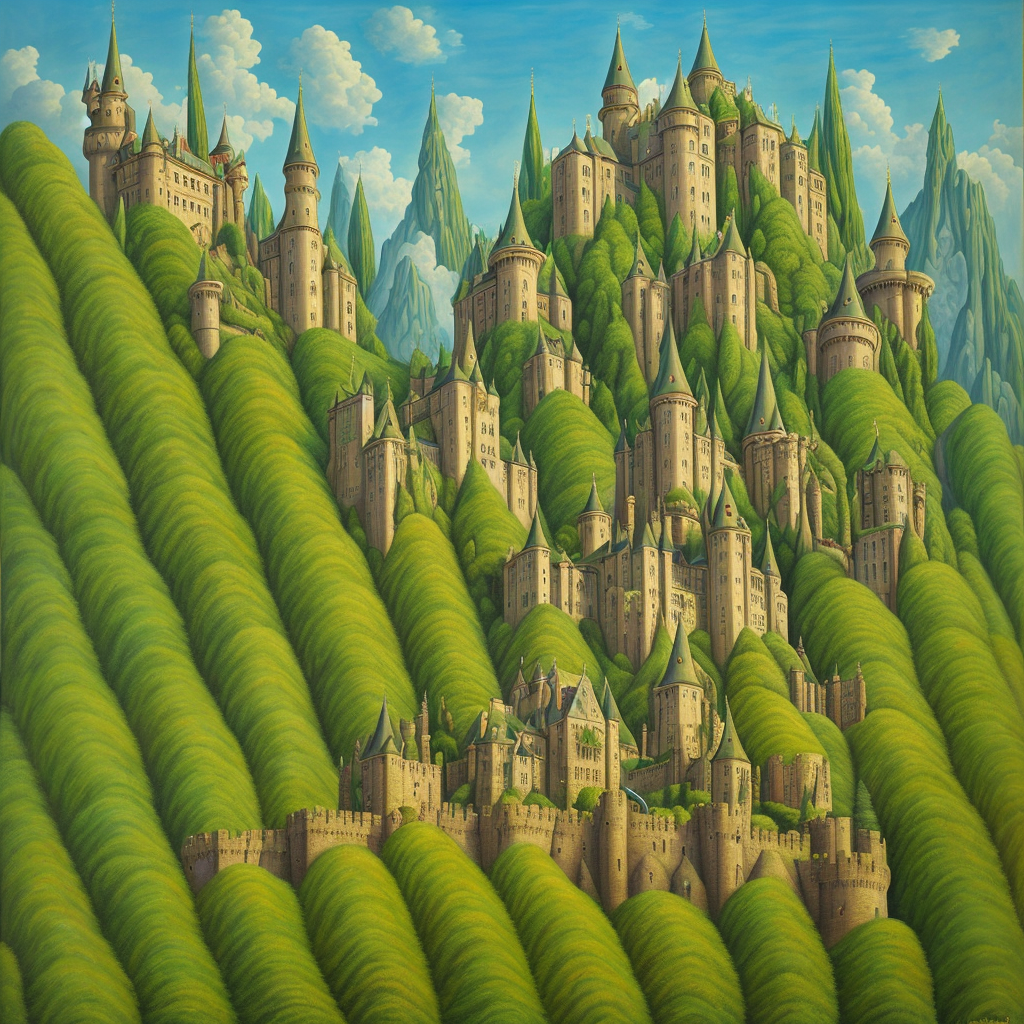
\includegraphics[width=1\textwidth]{/Users/nikolajprovorov/Yandex.Disk-368690@edu.itmo.ru.localized/Lab6_Furry_series/7.png}
    \caption{Картинка с гугл диска, которая мне очень приглянулась.}
    \label{fig:Source_img_1}
\end{figure}

Дальше по инструкции, работаем как сказано, но переписываем код под Python.

А вот и результат, мы получили фурье-образ изображения.

\begin{figure}[ht!]
    \centering
    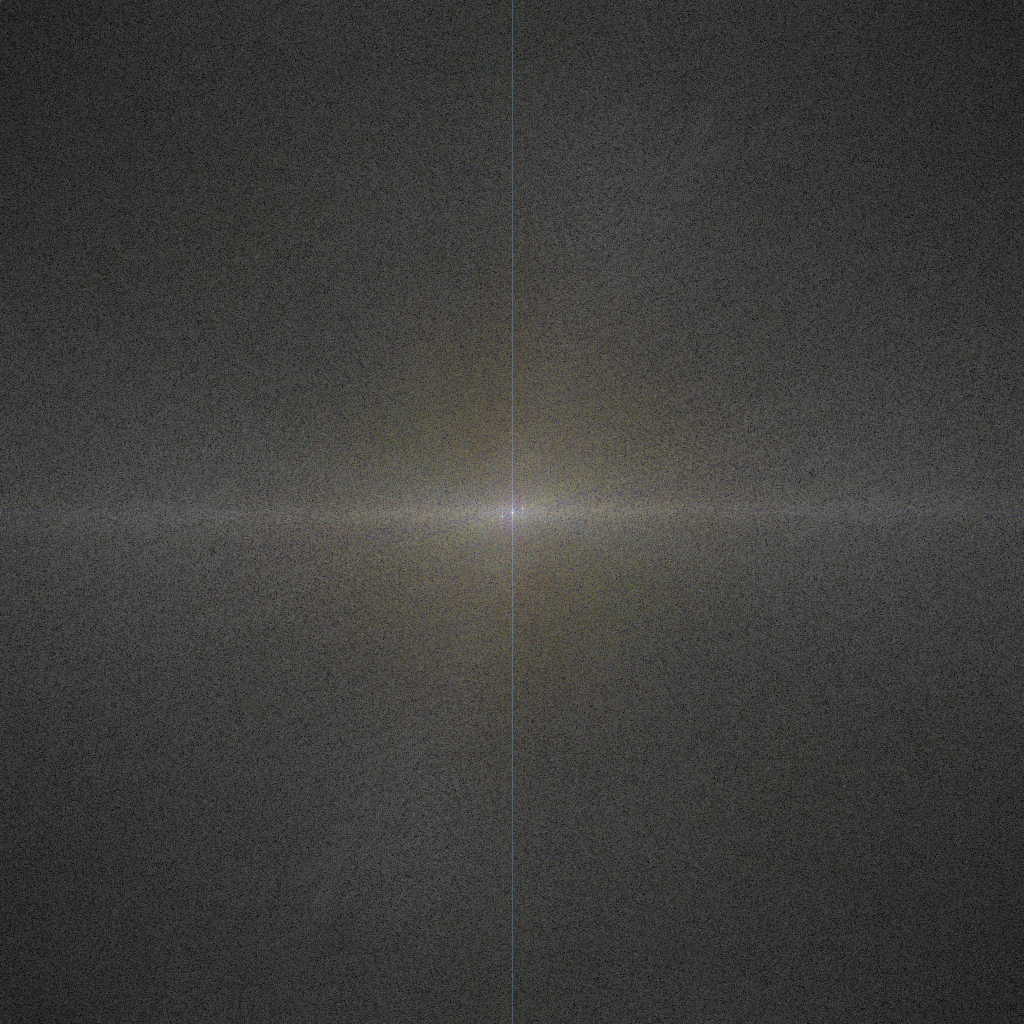
\includegraphics[width=1\textwidth]{/Users/nikolajprovorov/Yandex.Disk-368690@edu.itmo.ru.localized/Lab6_Furry_series/abs_fourier_log.png}
    \caption{Фурье-образ изображения.}
\end{figure}

\clearpage

На изображении присутсвует периодичность, которую мы можем убрать, если убрать пики. А вот и они:

\begin{figure}[ht!]
    \centering
    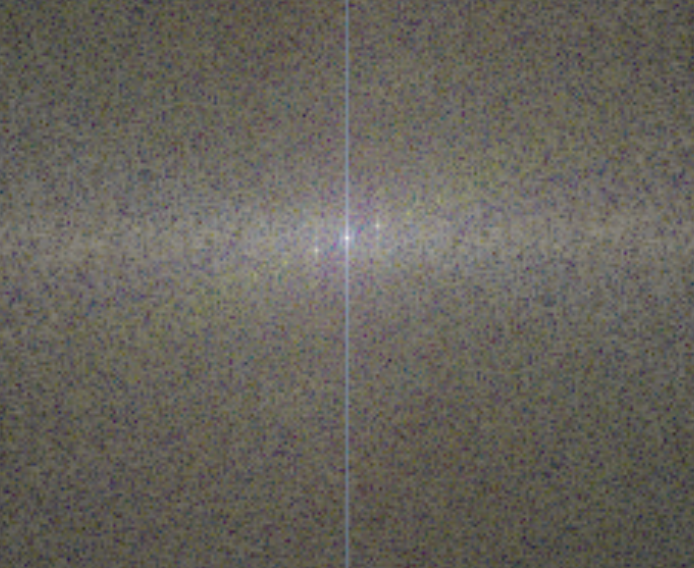
\includegraphics[width=1\textwidth]{/Users/nikolajprovorov/Yandex.Disk-368690@edu.itmo.ru.localized/Lab6_Furry_series/image.png}
    \caption{Пики.}
\end{figure}

Убрали в фотошопе, а вот и результат:

\clearpage

\begin{figure}[ht!]
    \centering
    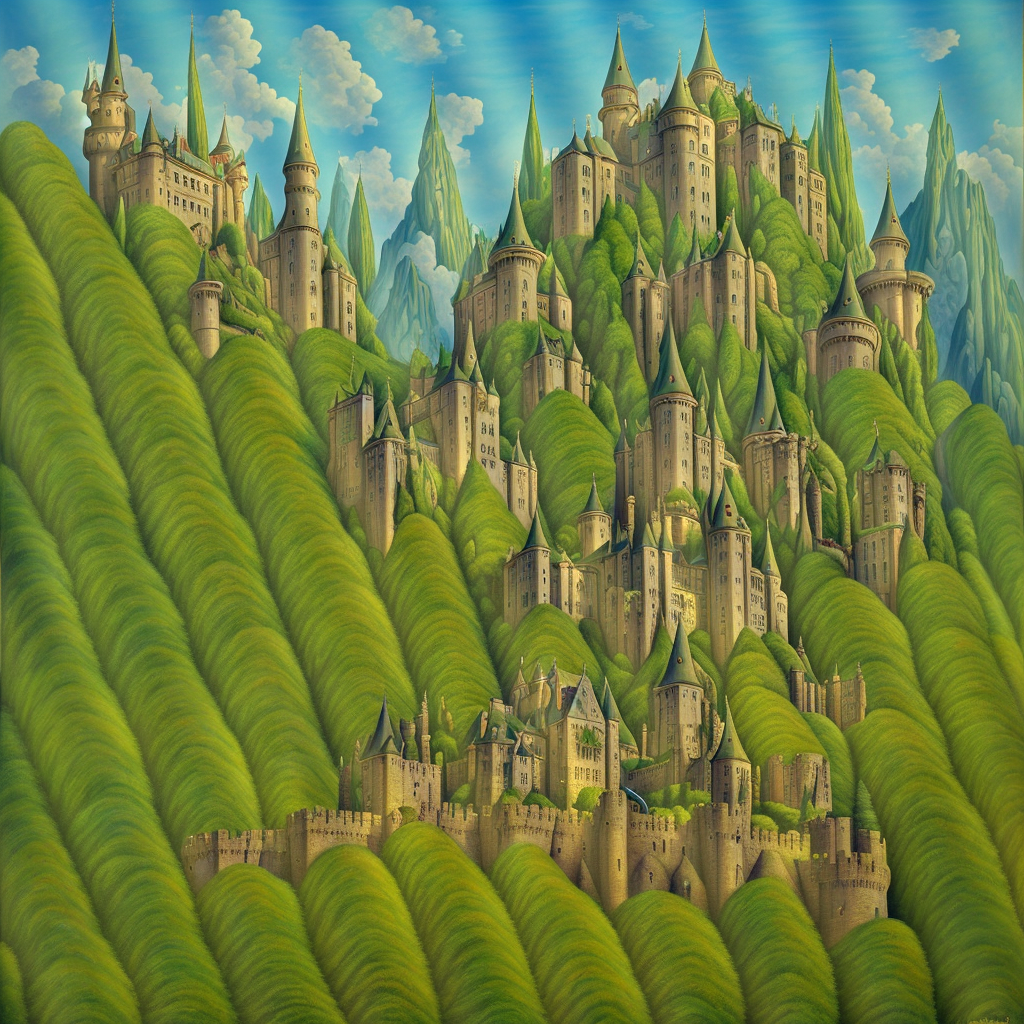
\includegraphics[width=1\textwidth]{/Users/nikolajprovorov/Yandex.Disk-368690@edu.itmo.ru.localized/Lab6_Furry_series/restored.png}
    \caption{Результат.}
\end{figure}

Стало лучше, и мне это нравится. Чуть изменилось само изображение, возможно мы затронули то, что не надо было, но уже ладно. Двигаемся дальше.



\clearpage

\section{Размытие изображения}

Для начала мы преобразуем изображение в черно-белое.

\begin{figure}[ht!]
    \centering
    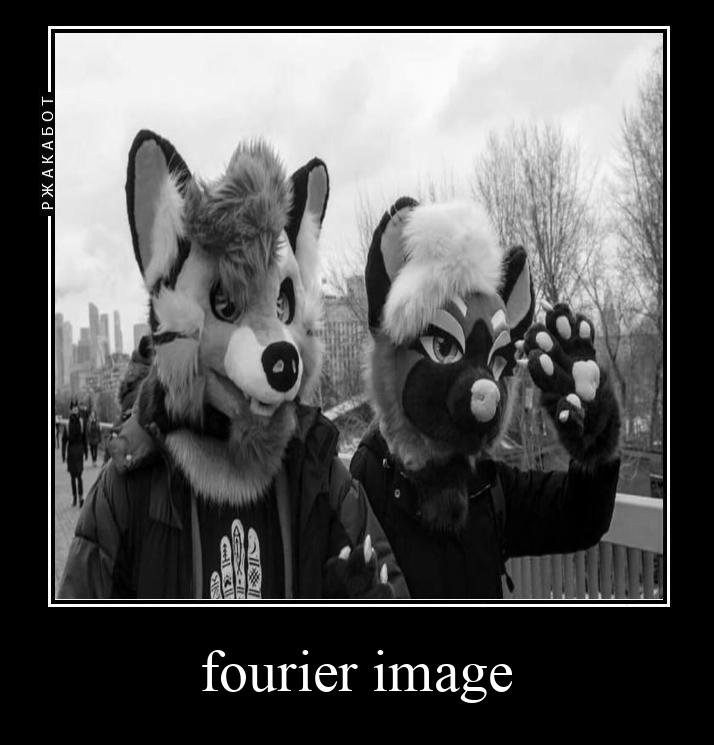
\includegraphics[width=0.5\textwidth]{/Users/nikolajprovorov/Yandex.Disk-368690@edu.itmo.ru.localized/Lab6_Furry_series/bw.png}
    \caption{Черно-белое изображение}
\end{figure}

Для начала выберу 3 нечетных значения $n = 3, 5, 7$

\subsection{Блочное размытие.}

Создадим 3 матрицы ядра блочного размытия. Для этого используем команду 

\begin{equation}
    ones(n)/(n^2)
\end{equation}

\clearpage

Посмотрим на результаты применения ядер к изображению.

\begin{figure}[ht!]
    \centering
    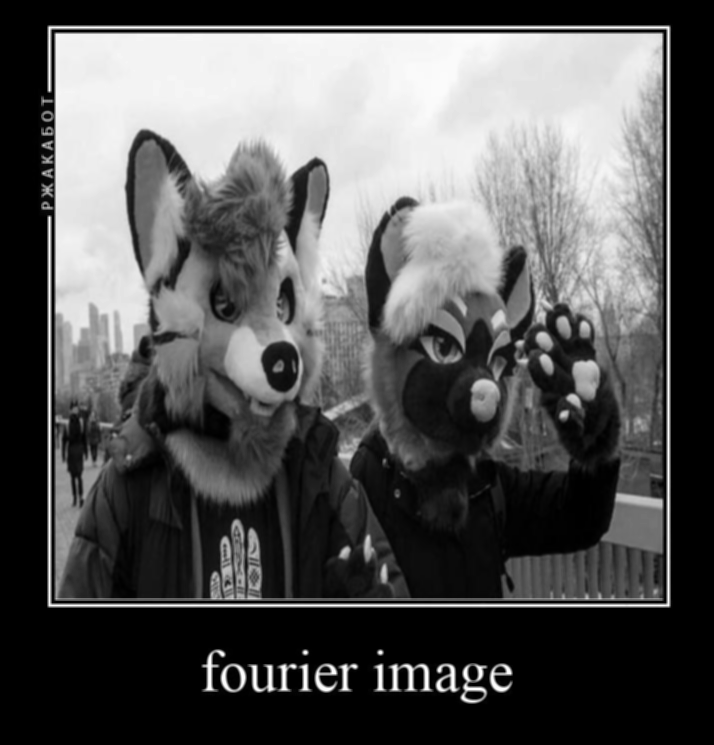
\includegraphics[width=0.5\textwidth]{/Users/nikolajprovorov/Yandex.Disk-368690@edu.itmo.ru.localized/Lab6_Furry_series/block_3.png}
    \caption{Блочное размытие с $n = 3$}
\end{figure}

\begin{figure}[ht!]
    \centering
    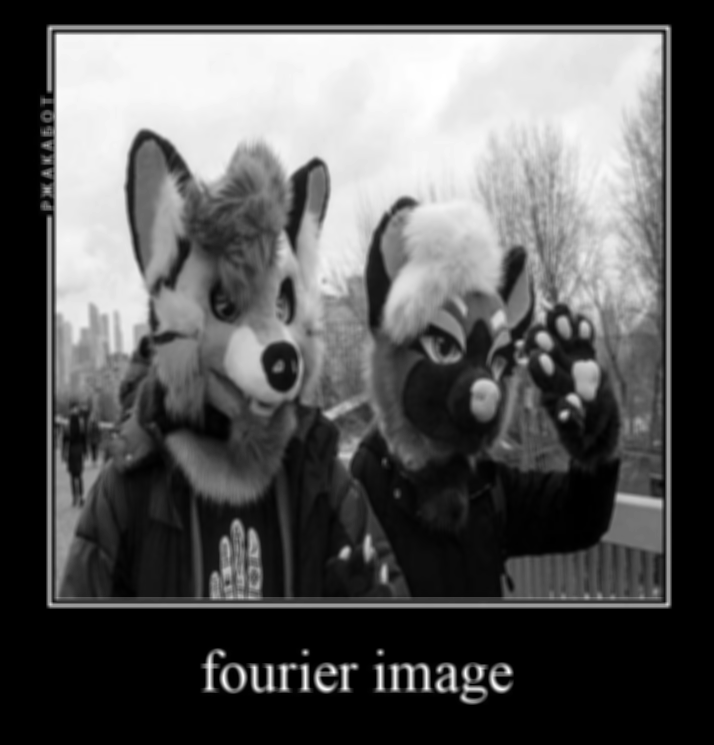
\includegraphics[width=0.5\textwidth]{/Users/nikolajprovorov/Yandex.Disk-368690@edu.itmo.ru.localized/Lab6_Furry_series/block_5.png}
    \caption{Блочное размытие с $n = 5$}
\end{figure}

\clearpage

\begin{figure}[ht!]
    \centering
    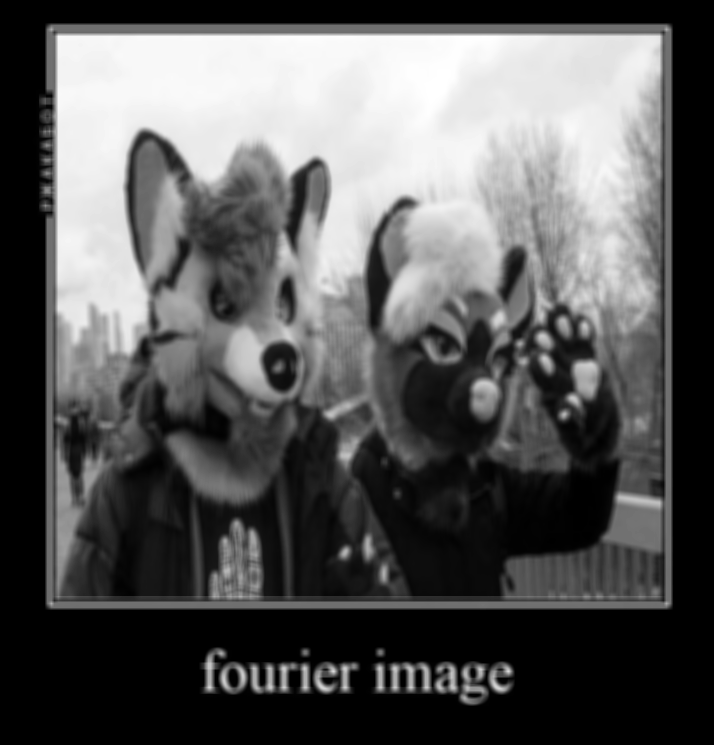
\includegraphics[width=0.5\textwidth]{/Users/nikolajprovorov/Yandex.Disk-368690@edu.itmo.ru.localized/Lab6_Furry_series/block_7.png}
    \caption{Блочное размытие с $n = 7$}
\end{figure}

\subsection{Размытие Гаусса.}

Применим фильтр Гаусса к изображению.

\begin{figure}[ht!]
    \centering
    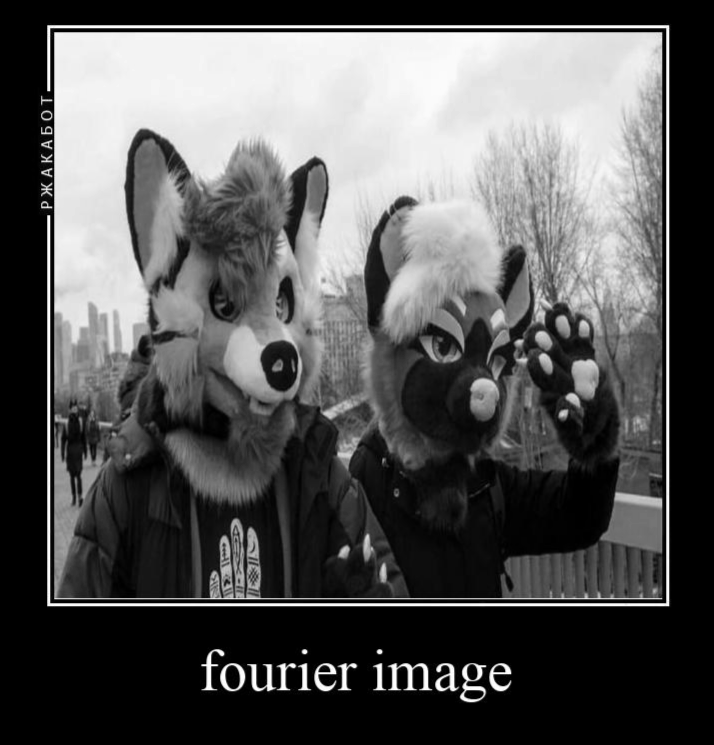
\includegraphics[width=0.5\textwidth]{/Users/nikolajprovorov/Yandex.Disk-368690@edu.itmo.ru.localized/Lab6_Furry_series/gaussian_3.png}
    \caption{размытие Гаусса с $n = 3$}
\end{figure}

\clearpage

\begin{figure}[ht!]
    \centering
    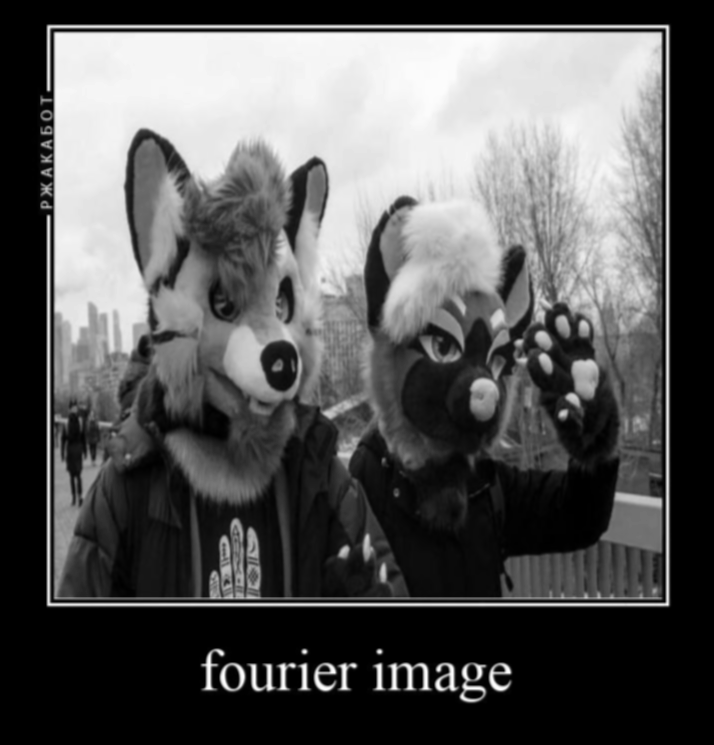
\includegraphics[width=0.5\textwidth]{/Users/nikolajprovorov/Yandex.Disk-368690@edu.itmo.ru.localized/Lab6_Furry_series/gaussian_5.png}
    \caption{размытие Гаусса с $n = 5$}
\end{figure}

\begin{figure}[ht!]
    \centering
    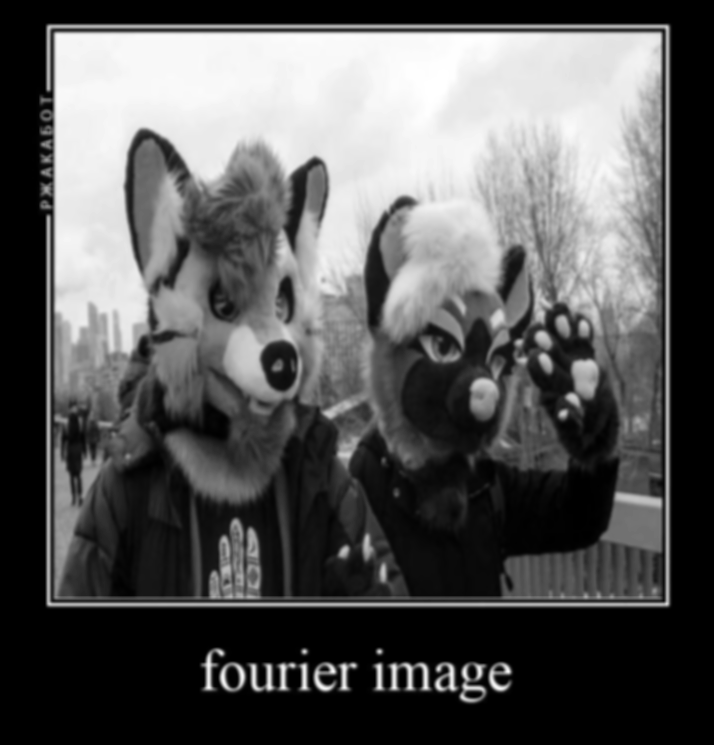
\includegraphics[width=0.5\textwidth]{/Users/nikolajprovorov/Yandex.Disk-368690@edu.itmo.ru.localized/Lab6_Furry_series/gaussian_7.png}
    \caption{размытие Гаусса с $n = 7$}
\end{figure}

\clearpage

Теперь посмотрм что там с фурье-котовасией.

\begin{figure}[ht!]
    \centering
    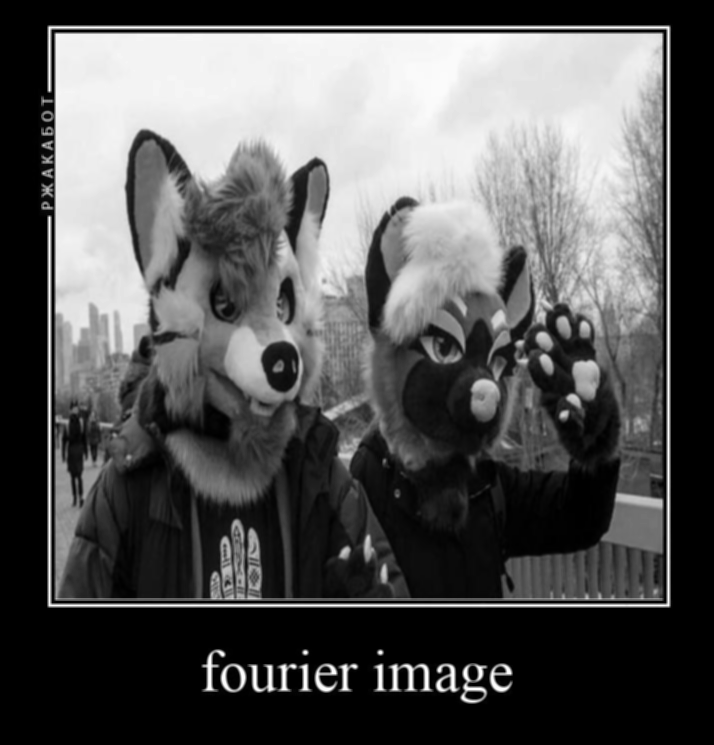
\includegraphics[width=0.5\textwidth]{/Users/nikolajprovorov/Yandex.Disk-368690@edu.itmo.ru.localized/Lab6_Furry_series/block_3.png}
    \caption{Блочное размытие с $n = 3$ (через фурье)}
\end{figure}

\begin{figure}[ht!]
    \centering
    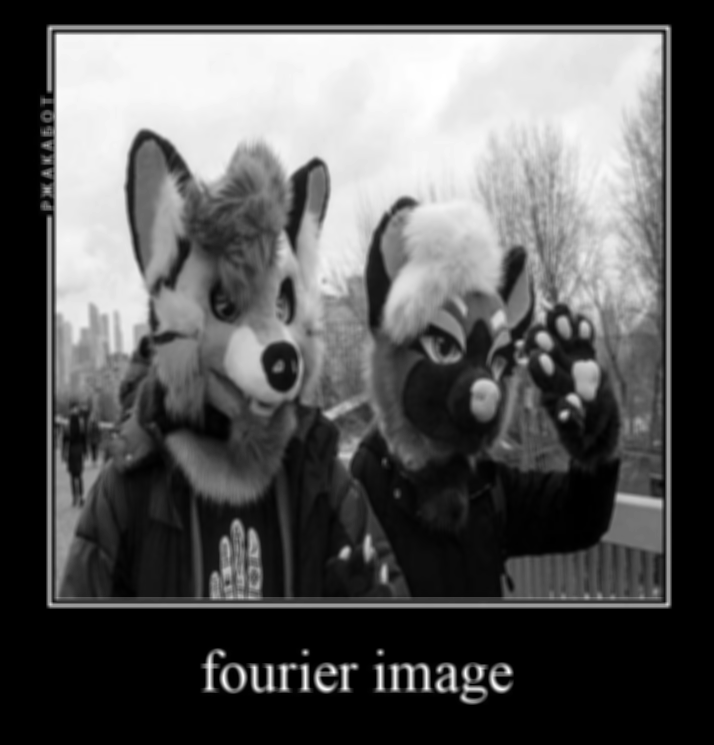
\includegraphics[width=0.5\textwidth]{/Users/nikolajprovorov/Yandex.Disk-368690@edu.itmo.ru.localized/Lab6_Furry_series/block_5.png}
    \caption{Блочное размытие с $n = 5$ (через фурье)}
\end{figure}

\clearpage

\begin{figure}[ht!]
    \centering
    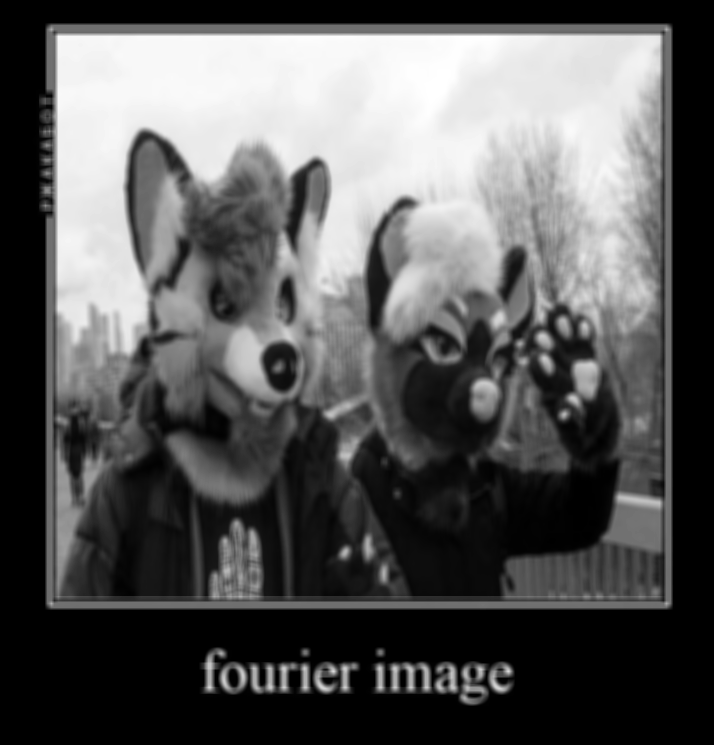
\includegraphics[width=0.5\textwidth]{/Users/nikolajprovorov/Yandex.Disk-368690@edu.itmo.ru.localized/Lab6_Furry_series/block_7.png}
    \caption{Блочное размытие с $n = 7$ (через фурье)}
\end{figure}

\begin{figure}[ht!]
    \centering
    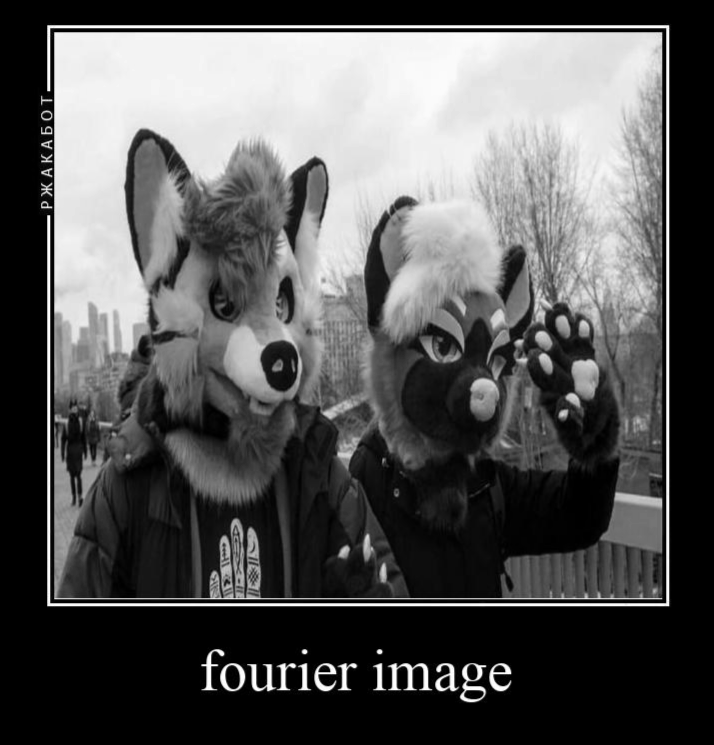
\includegraphics[width=0.5\textwidth]{/Users/nikolajprovorov/Yandex.Disk-368690@edu.itmo.ru.localized/Lab6_Furry_series/gaussian_3.png}
    \caption{размытие Гаусса с $n = 3$ (через фурье)}
\end{figure}

\clearpage

\begin{figure}[ht!]
    \centering
    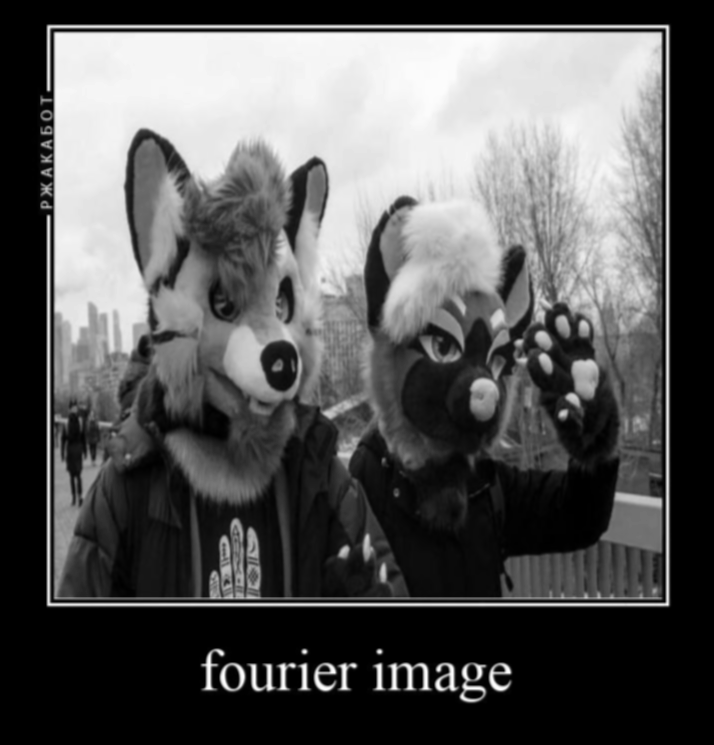
\includegraphics[width=0.5\textwidth]{/Users/nikolajprovorov/Yandex.Disk-368690@edu.itmo.ru.localized/Lab6_Furry_series/gaussian_5.png}
    \caption{размытие Гаусса с $n = 5$ (через фурье)}
\end{figure}

\begin{figure}[ht!]
    \centering
    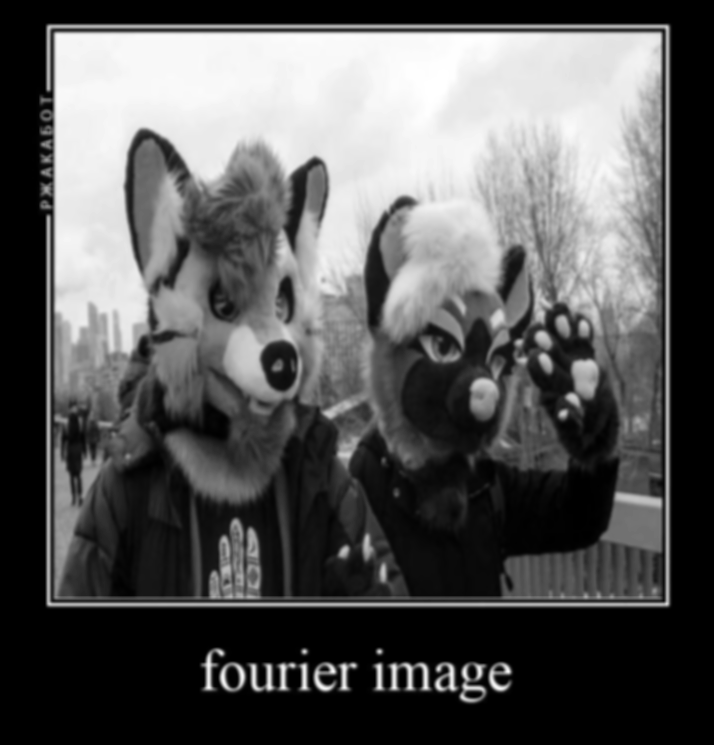
\includegraphics[width=0.5\textwidth]{/Users/nikolajprovorov/Yandex.Disk-368690@edu.itmo.ru.localized/Lab6_Furry_series/gaussian_7.png}
    \caption{размытие Гаусса с $n = 7$ (через фурье)}
\end{figure}

Результаты совпадают, прикольно. Все работает.

Если сравнивать блочное размытие с Гауссом, то можно заметить, что Гауссовское размытие более плавное, чем блочное. Также Гауссовское размытие не так сильно ухудшает качество изображения, как блочное.

\clearpage

\section{Увеличение резкости изображения}

Для начала мы преобразуем изображение в черно-белое.

\begin{figure}[ht!]
    \centering
    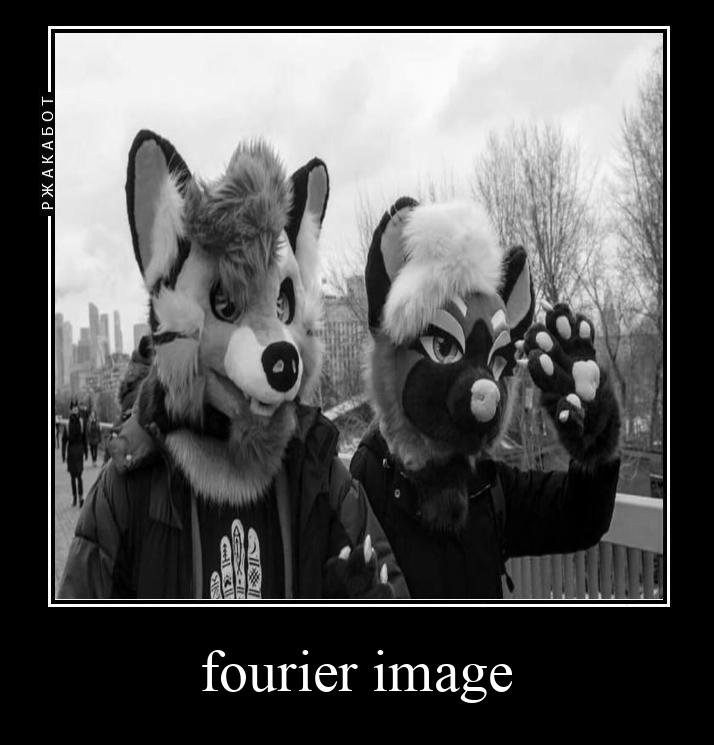
\includegraphics[width=0.5\textwidth]{/Users/nikolajprovorov/Yandex.Disk-368690@edu.itmo.ru.localized/Lab6_Furry_series/bw.png}
    \caption{Черно-белое изображение}
\end{figure}

Зададим матрицу ядра увеличния резкости:

\begin{equation}
    K = 
    \begin{bmatrix}
        0 & -1 & 0 \\
        -1 & 5 & -1 \\
        0 & -1 & 0
    \end{bmatrix}
\end{equation}

Посмотрим на результат применения:

\clearpage

\begin{figure}[ht!]
    \centering
    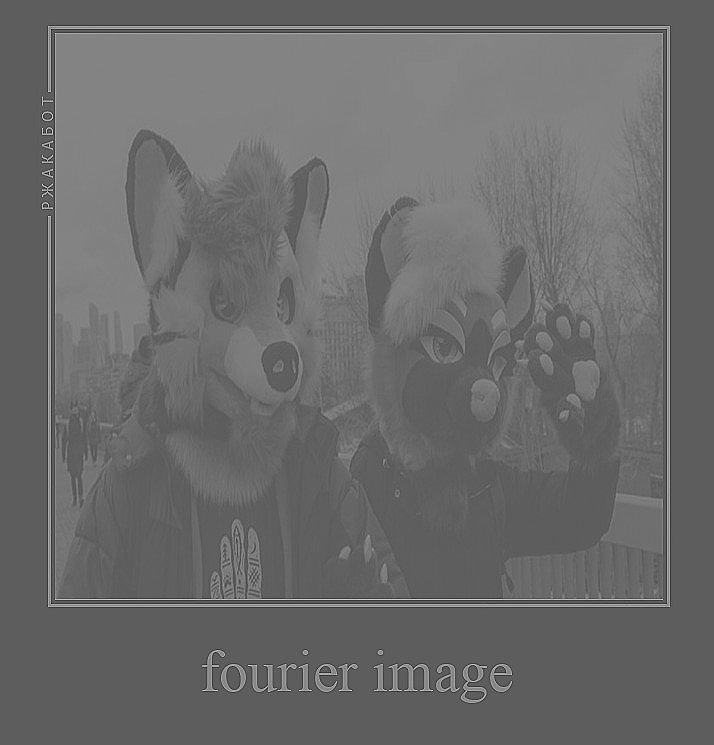
\includegraphics[width=0.5\textwidth]{/Users/nikolajprovorov/Yandex.Disk-368690@edu.itmo.ru.localized/Lab6_Furry_series/laplacian.png}
\end{figure}

Стало явно лучше, резкость увеличилась, но изображение потеряло в контрасте.

Давайте посмотрим теперь на результат всего вот того фурье:

\begin{figure}[ht!]
    \centering
    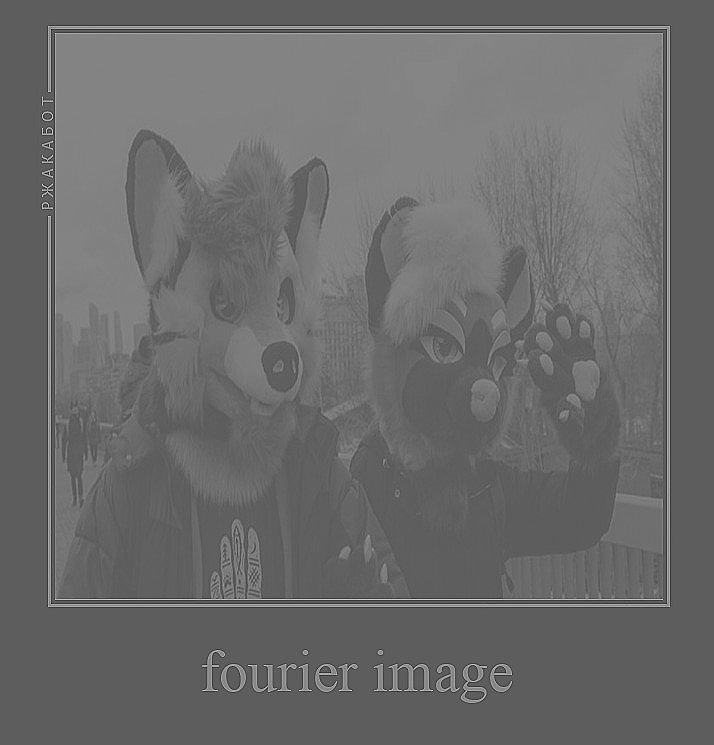
\includegraphics[width=0.5\textwidth]{/Users/nikolajprovorov/Yandex.Disk-368690@edu.itmo.ru.localized/Lab6_Furry_series/laplacian.png}
    \caption{Увеличение резкости изображения что-то там фурье}
\end{figure}

О, прикол, совпали. Теорема о свертке работает корректно.

\clearpage

\section{Выделение краев изображения}

Для начала мы преобразуем изображение в черно-белое.

\begin{figure}[ht!]
    \centering
    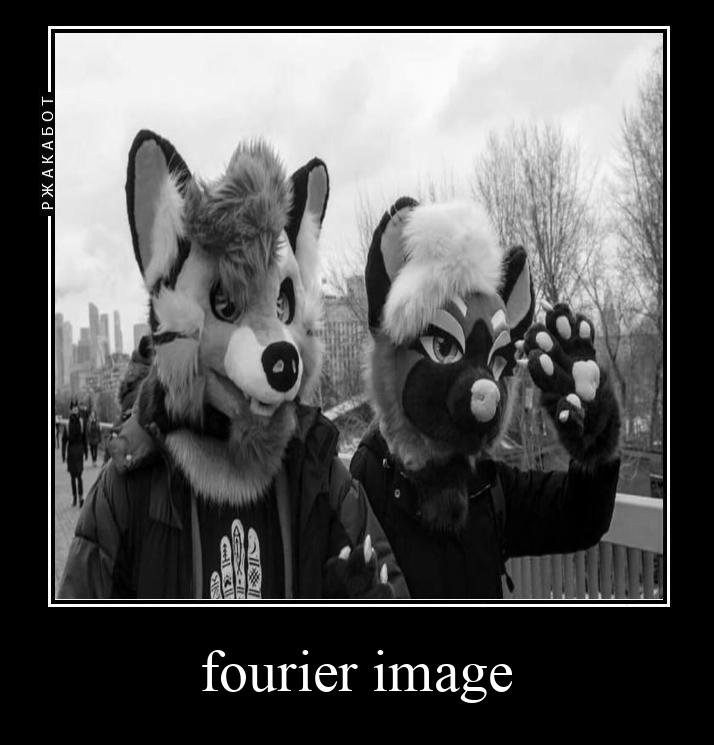
\includegraphics[width=0.5\textwidth]{/Users/nikolajprovorov/Yandex.Disk-368690@edu.itmo.ru.localized/Lab6_Furry_series/bw.png}
    \caption{Черно-белое изображение}
\end{figure}

Зададим матрицу ядра выделения краев:

\begin{equation}
    K = 
    \begin{bmatrix}
        -1 & -1 & -1 \\
        -1 & 8 & -1 \\
        -1 & -1 & -1
    \end{bmatrix}
\end{equation}

Найдем свертку исходного изображения с ядром и тд и тп, короче вот результат:

\clearpage

\begin{figure}[ht!]
    \centering
    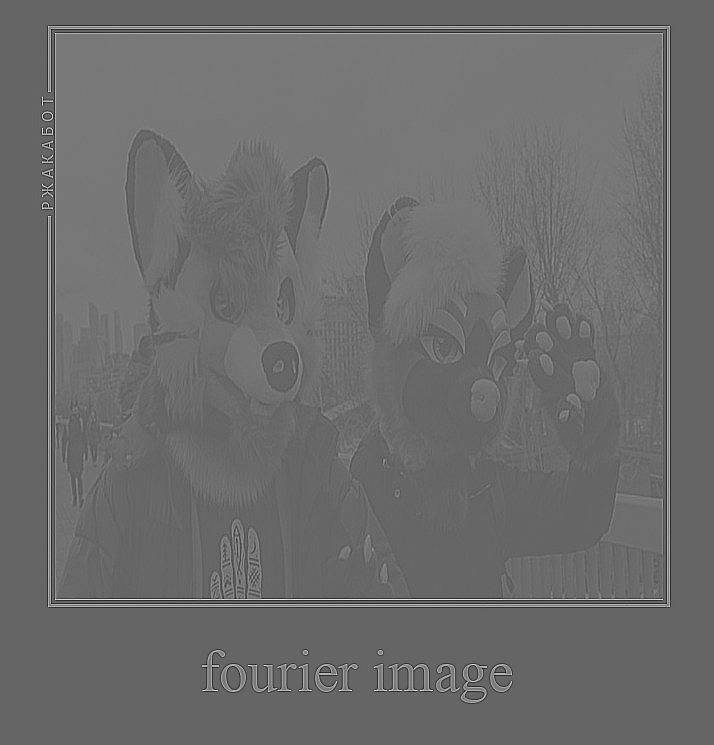
\includegraphics[width=0.5\textwidth]{/Users/nikolajprovorov/Yandex.Disk-368690@edu.itmo.ru.localized/Lab6_Furry_series/edge_x.png}
    \caption{Выделение краев изображения}
\end{figure}

Ну получилось очень даже неплохо, контрастность конечно пострадала, и сильно, но зато какие края!

Давайте посмотрим теперь на результат всего вот того фурье:

\begin{figure}[ht!]
    \centering
    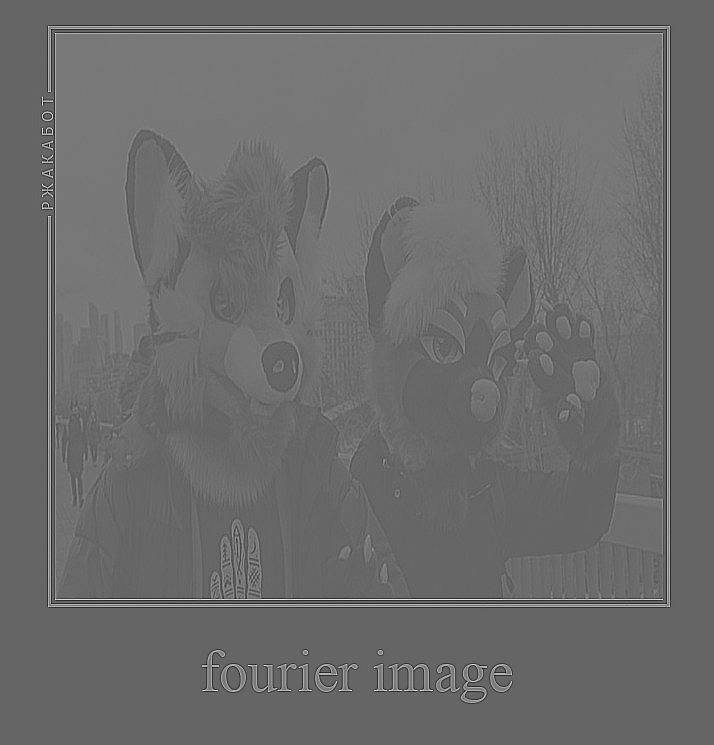
\includegraphics[width=0.5\textwidth]{/Users/nikolajprovorov/Yandex.Disk-368690@edu.itmo.ru.localized/Lab6_Furry_series/edge_x.png}
    \caption{Выделение краев изображения}
\end{figure}

О, прикол, совпали. Теорема о свертке работает корректно.

\clearpage

В целом, так как это последняя лабораторная по данному предмету, хочу сказать вам спасибо. 

\begin{figure}[ht!]
    \centering
    
\includegraphics[width=1\textwidth]{/Users/nikolajprovorov/Yandex.Disk-368690@edu.itmo.ru.localized/Lab6_Furry_series/Unknown.jpeg}
    \caption{Спасибо за внимание.}
\end{figure}